% !TEX root = ../thesis-example.tex
%
\pagestyle{empty}
\hfill
\vfill
\pdfbookmark[0]{Colophon}{Colophon}
\section*{Appendix}\label{sec:appendix}

\subsection{Assumptions}\label{sec:appendix:assumptionssong}
In the paper and in the following proofs, we make the following assumptions :
\begin{enumerate}
    \item $p(\vx) \in \cal C^2(\reals^d)$ and $\E_P\left[\Vert \vx \Vert_2^2\right] < \infty$.
    \item $q(\vx) \in \cal C^2(\reals^d)$ and $\E_Q\left[\Vert \vx \Vert_2^2\right] < \infty$.
    \item $\forall t \in [0, T]$, $\vf(\vx, t) \in \cal C^1(\Xset)$ and $\exists C>0$ such that $\forall \vx \in \reals^d,t\in[0, T],\Vert \vf(\vx, t)\Vert_2 \leq C( 1+\Vert\vx\Vert_2)$. 
    \item $\exists C >0 $ such that $\forall \vx, \vy \in \reals^d, \ \Vert \vf(\vx, t) - \vf(\vy, t)\Vert_2 \leq C\Vert \vx - \vy\Vert_2$.
    \item $g\in \cal C^1([0, T])$ and $\forall t \in [0, T],\ \vert g(t)\vert > 0$.
    \item For any open bounded set $\cal O \subset \reals^d$, $\int_0^T \int_{\cal O} \Vert p_t(\vx_t) \Vert_2^2 + d\Vert \nabla_{\vx_t}p_t(\vx_t) \Vert_2^2\d \vx_t \d t < \infty$.
    \item $\exists C >0$ such that $\forall \vx\in \reals^d, t\in[0,T]:\ \Vert\nabla_{\vx_t} \log p_t(\vx_t)\Vert_2 \leq C(1+\Vert \vx_t\Vert_2)$.
    \item $\exists C >0$ such that $\forall \vx,\vy\in \reals^d,t\in[0,T]:\ \Vert\nabla_{\vx_t} \log p_t(\vx_t) - \nabla_{\vx_t} \log p_t(\vy_t)\Vert_2 \leq C\Vert \vx_t - \vy_t\Vert_2$.
    \item $\exists C>0$ such that $\forall \vx\in \reals^d, t\in[0,T]:\ \Vert\nabla_{\vx_t} \vs_\theta(\vx_t, t)\Vert_2 \leq C(1+\Vert \vx_t\Vert_2)$.
    \item $\exists C>0$ such that $\forall \vx,\vy\in \reals^d,t\in[0,T]:\ \Vert\nabla_{\vx_t} \vs_\theta(\vx_t, t) - \nabla_{\vx_t} \vs_\theta(\vy_t, t)\Vert_2 \leq C\Vert \vx_t - \vy_t\Vert_2$.
    \item Nokitov's condition: $\E_P\left[\exp\left(\frac{1}{2}\int_0^T\Vert \nabla_{\vx_t} \log p_t(\vx_t)-\vs_\theta(\vx_t, t)\Vert_2^2\d t\right)\right] < \infty$.
    \item  $\forall t\in[0, T], \exists k>0: \ p_t(\vx)=O(e^{-\Vert \vx \Vert_2^k})$ as $\Vert \vx \Vert_2 \to \infty$.
\end{enumerate}

\begin{theorem}\citep{kim2023refininggenerativeprocessdiscriminator}
    Suppose that the score network $s_{\theta}$ satisfies assumption \ref{ass:elbo}. Then $s_{\theta} \in S_{\mathrm{sol}}$. We thus denote by $\Hat{P}_{t}$ the distribution with density $\Hat{p}_{t}(x)$ such that $s_{\theta}(x,t) = \nabla \log \Hat{p}_{t}(x)$
\end{theorem}



\begin{theorem}\citep{kim2023refininggenerativeprocessdiscriminator}
Suppose that assumption \ref{ass:elbo} is satisfied by the estimated score network $s_{\theta}$. Suppose in addition that $s_{\theta}(x,T) = \nabla \log \pi(x)$.
Then, by noting $c_{\theta}(x,t) = \nabla \log p_{t}(x) - s_{\theta}(x,t) = \nabla \log \frac{p_{t}(x)}{s_{\theta}(x,t)}$, the backward SDE defined by : 
\begin{equation}\label{eq:refined_backward_SDE}
    dx = f(x,t) - \frac{1}{2}g(t)^{2}(s_{\theta}(x,t) + c_{\theta}(x,t))dt
\end{equation}
coincides with the backward SDE of the diffusion process induced by the target distribution (Equation \ref{eq:backward_diffusion}).  
\end{theorem}



\subsection{Proof of Theorem \ref{theorem:exploding_kl}}\label{app:sec:proofsuboptimal}



\begin{theorem*}
    Let $\left\{\vx(t)\right\}_{t\in[0, T]}$ be a diffusion process defined by Equation~\eqref{eq:forward_diff}. Assume that $P$ and $\whP$ satisfy the assumptions detailed in Appendix~\ref{sec:appendix:assumptionssong}. Then, for every $\varepsilon>0$ and for every $\delta>0$, there exists a discriminator $\vd:\reals^d\times\reals\to\reals$ trained to minimize the cross-entropy such that:
\begin{equation}
    \calL_{\mathrm{CE}}^{d}(\phi)\leq \varepsilon \et \KL(P\Vert \widetilde{P}) \geq \delta,
\end{equation}
where $\widetilde{P}$ is the distribution induced by discriminator guidance with $\vd$.
\end{theorem*}



\subsubsection{Finding a problematic case}
The aim of discriminator guidance is to minimize the Kullback-Leibler divergence between the target distribution $P$, and the refined distribution $\tilde{P}$.
Following the assumptions detailed in Appendix \ref{sec:appendix:assumptionssong}, this quantity can be written as : 
\begin{align}
    \KL(P\Vert \wtP) = \KL(P_T\Vert Q) + \int_0^Tg(t)^2\E_{P_t}\left[\Vert \nabla_{\vx_t} \log p_t(\vx_t) - \vs_\theta(\vx_t, t) - \nabla_{\vx_t}\vd_\phi(\vx_t, t)\Vert_2^2 \right]\dt.
\end{align}
Thus, discriminator guidance minimizes the latter term of the equality, that we denote as :


\begin{align}\label{main-goal}
    E_{\phi} =\int_0^Tg(t)^2\E_{P_t}\left[\Vert \nabla_{\vx_t} \log p_t(\vx_t) - \vs_\theta(\vx_t, t) - \nabla_{\vx_t}\vd_\phi(\vx_t, t)\Vert_2^2 \right]\dt.
\end{align}
where $d_{\phi}(\vx_{t})$ is the estimated density ratio by training the discriminator $d_{\phi}$.

We consider the case of estimating $d_{\phi}$ by minimizing the cross-entropy up to $\varepsilon$. We would like to find a pathological case where this would not minimize the mean square error in Equation \ref{main-goal}.
The estimation error of the discriminator can be derived from the duality difference in estimating the g-Bregman divergence, with : 
\begin{align}
    g(\vx) = u\log(u) + (u+1)\log(u+1)
\end{align}
We denote by $\mathcal{D}_{g}(P \Vert P') = \inf_{f \in \mathcal{M}} \mathbb{E}_{(\vx) \sim p_{t}}\left[\log(\sigma(f(\vx_{t})))\right] - \mathbb{E}_{\vx \sim \hat{p}_{t}}\left[-\log(1 - \sigma(f(\vx_{t})))\right]$, where $\mathcal{M}$ denotes the set of all measurable functions. This quantity estimates the optimal cross-entropy that any measurable density ratio estimator $f$ can achieve.

The estimated $d_{\phi}$ has minimized the following quantity $\mathcal{D}_{g}^{\phi} = inf_{\omega \in R^{N}}\mathbb{E}_{\vx \sim p_{t}}\left[\log(\sigma(T_{\omega}(\vx_{t})))\right] - \mathbb{E}_{\vx \sim \hat{p}_{t}}\left[-\log(1 - \sigma(T_{\omega}(\vx_{t})))\right]$. We use the results of \citep{uehara_generative_2016,sugiyama_density_nodate,verine2024precision} to compute the estimation error of the cross-entropy : 

\begin{theorem*}
    For any discriminator $T_{\phi} : \mathcal{X} \xrightarrow{} R$ and density ratio estimation $d_{\phi} = \nabla_{\vx_t} g^{*}(T_{\phi}(\vx))$, we have :
\begin{align}\label{thm1}
    D_{g}(P||\hat{P}) - D_{g}^{\phi}(P||\hat{P}) = \mathbb{E}_{\hat{P}}
    \left[
    \text{Breg}_{g}\left(d_{\phi}(\vx),\frac{p(\vx)}{\hat{p}(\vx)}\right)
    \right]
\end{align}
where $g*$ denotes the Fenchel conjugate of $g$.
\end{theorem*}

Suppose a discriminator was trained on minimizing the cross-entropy $D_{\text{g}}^{\phi}$ such that it is $\varepsilon$-close to the optimal cross-entropy $D_{\text{g}}$. Thus, we can write : \begin{equation} \label{eq:bregmaneps}
D_{g}(P \Vert \hat{P}) - D_{g}^{\phi}(P \Vert \hat{P}) \leq \varepsilon
\end{equation}
We consider the case when, for all $(\vx) \sim \hat{P}$, $\text{Breg}_{g}(d_{\phi}(\vx),\frac{p(\vx)}{\hat{p}(\vx)}) \leq \varepsilon$
Suppose moreover that the estimated density ratio $d_{\phi}(\vx) = \frac{p(\vx)}{\hat{p(\vx)}} + h(\vx)$. We also note $\frac{p(\vx)}{\hat{p(\vx)}} = r_{\opt}(\vx)$. Thus, we can write, for $\vx \in \mathbb{R}$:
\[
\text{Breg}_{g}\left(d_{\phi}(\vx),\frac{p(\vx)}{\hat{p}(\vx)}\right) = g(d_{\phi}(\vx)) - g(r_{\opt}(\vx)) - \nabla_{\vx_t} g(r_{\opt}(\vx))(d_{\phi}(\vx) - r_{\opt}(\vx)))
\]
With : 
\begin{align}
g(d_{\phi}(\vx)) &=\begin{aligned}[t] (r_{\opt}(\vx)& + h(\vx))\log(r_{\opt}(\vx) + h(\vx))\\
&- (r_{\opt}(\vx) + h(\vx) +1 )\log(r_{\opt}(\vx) + h(\vx) +1)\end{aligned}
    \\
    &=\begin{aligned}[t]
        (r_{\opt}(\vx)& + h(\vx))\log (r_{\opt}(\vx)) \\
        &+ (r_{\opt}(\vx) + h(\vx))\log\left(1+ \frac{h(\vx)}{r_{\opt}(\vx)}\right) \\
        &- (r_{\opt}(\vx) + h(\vx) +1)\log(r_{\opt}(\vx) + h(\vx) +1)\end{aligned}
    \\
    &\leq
    \begin{aligned}&(r_{\opt}(\vx) + h(\vx))\log(r_{\opt}(\vx)) + (r_{\opt}(\vx)+h)\frac{h(\vx)}{r_{\opt}(\vx)}  \\
    &- (r_{\opt}(\vx) + h(\vx) +1)\log(r_{\opt}(\vx) + h(\vx) +1)\end{aligned}
    \label{eq:dl}
\end{align}
Moreover,
\begin{align}
g(r_{\opt}(\vx)) &= r_{\opt}(\vx)\log(r_{\opt}(\vx)) + (r_{\opt}(\vx) +1)\log(r_{\opt}(\vx)+1)\label{eq:sec-part} \end{align}
and the third term is given by 
\begin{align}
\nabla_{\vx_t} g(r_{\opt}(\vx))(d_{\phi}(\vx) - r_{\opt}(\vx))) &= (\log(r_{\opt}(\vx)) - \log(r_{\opt}(\vx)+1))h(\vx)\label{eq:grad-part}
\end{align}
Inequality \ref{eq:dl} results from the Taylor expansion of $\log(1+(\vx))$ when $(\vx)$ is close to zero, as $\log(1+(\vx)) \leq (\vx)$.
By summing the expressions \ref{eq:dl},\ref{eq:sec-part},\ref{eq:grad-part}, we obtain an upper bound on the $g$-Bregman divergence between the true and estimated density ratio : 
\begin{align}
    \text{Breg}_{g}\left(d_{\phi}(\vx),r_{\opt}(\vx)\right) &\leq 
    \begin{aligned}[t]
    &\left(1+\frac{h^{2}(\vx)}{r_{\opt}(\vx)} \right) + \left(r_{\opt}(\vx) +1 \right) \log\left( r_{\opt}+1\right) + h(\vx)\log\left(r_{\opt}(\vx) +1 \right)  \\
    &- \left(r_{\opt}(\vx) + h(\vx) + 1\right)\log\left( r_{\opt}(\vx) + h(\vx) + 1\right)\end{aligned}
    \\
    &=\begin{aligned}[t]
    &\left(h(\vx) + r_{\opt}(\vx)\right)\frac{h(\vx)}{r_{\opt}(\vx)}   \\
    &+\left[r_{\opt}(\vx) + h(\vx) + 1\right]\left[\log(r_{\opt}(\vx)+1) - \log(\left(r_{\opt}(\vx) + h(\vx) + 1\right))  \right]
    \end{aligned}
    \\
    &=\begin{aligned}[t]
    (h(\vx) &+ r_{\opt}(\vx))\frac{h(\vx)}{r_{\opt}(\vx)}  \\
    & +\left(r_{\opt}(\vx) + h(\vx) + 1\right)\log\left( 1 - \frac{h(\vx)}{r_{\opt}(\vx) + h(\vx) + 1}\right)
    \end{aligned}
    \\
    &\leq
    \begin{aligned}
    (h(\vx) + r_{\opt}(\vx))\frac{h(\vx)}{r_{\opt}(\vx)} 
    - (r_{\opt}(\vx) + h(\vx) +1)\frac{h(\vx)}{r_{\opt}(\vx)+h(\vx) + 1}
    \end{aligned}
    \\
    &\leq \frac{h(\vx)^{2}}{r_{\opt}(\vx)}
\end{align}
One particular case of satisfaction of inequality \ref{eq:bregmaneps} is when all the elements in the expectation $\mathbb{E}_{\hat{P}}$ are below $\varepsilon$, that is when : \begin{align}
    \frac{h^{2}(\vx)}{r_{\opt}(\vx)} &\leq \varepsilon \\
    \Rightarrow h(\vx) &\leq \sqrt{\varepsilon r_{\opt}(\vx)}
\end{align}
This bound is notably satisfied for $h(\vx) = \sin(\omega \vx)\sqrt{\varepsilon r_{opt}(\vx)} $, $\forall \omega \in \mathbb{R}$
\subsubsection{Computing the gain}
We will now show that the value of the $E_\phi$ (c.f Equation \ref{main-goal}) can go to infinity for an estimated density ratio that has an $\varepsilon$-optimal cross-entropy. For this, we write, for $r(\vx) = r_{opt}(\vx) + h(\vx)$, with $h(\vx) =\sin(\omega (\vx))\sqrt{\varepsilon r_{opt}(\vx)} $ :
This bound is notably satisfied for $h(\vx) = \sin(\omega (\vx))\sqrt{\varepsilon r_{\opt}(\vx)} $, $\forall \omega \in \mathbb{R}$
\subsection{Computing the gain}
We will now show that the value of the gain (c.f Equation \ref{main-goal}) can go to infinity for an estimated density ratio that has an $\varepsilon$-optimal cross-entropy. For this, we compute, for $d_{\phi}(\vx) = r_{\opt}(\vx) + h(\vx)$, with $h(\vx) =\sin(\omega (\vx))\sqrt{\varepsilon r_{\opt}(\vx)} $ :
\begin{align}
    \nabla_{\vx_t} \log(d_{\phi}(\vx)) = \nabla_{\vx_t} \log(r_{\opt}(\vx)) + \nabla_{\vx_t} \log\left( 1 + \sqrt{\frac{\varepsilon}{r_{\opt}(\vx)}} \sin(\omega (\vx)) \right)
\end{align}
Moreover, we have : 
\begin{align}
    \nabla_{\vx_t} \log\left( 1 + \sqrt{\frac{\varepsilon}{r_{\opt}(\vx)}} \sin(\omega (\vx)) \right) = \frac{\sqrt{\varepsilon}\left(
    -\frac{1}{2}\nabla_{\vx_t} r_{\opt}(\vx)r_{\opt}^{-\frac{3}{2}}\sin(\omega (\vx)) + \sqrt{\frac{\varepsilon}{r_{\opt}(\vx)}} \omega \cos(\omega (\vx))
    \right)}{1 + \sqrt{\frac{\varepsilon}{r_{\opt}(\vx)}} \sin(\omega (\vx))}
\end{align}
Thus, the gain for a fixed timestep t is given by : 
\begin{align}
    E_{\phi}^{t} &=\begin{aligned} 
    \mathbb{E}_{P_{t}}\left[ 
    ||\nabla_{\vx_t} log (r_{\opt}(\vx)) - \nabla_{\vx_t} \log d_{\phi}(\vx) ||_{2}^{2}
    \right] 
    \end{aligned}
    \\
    &=\begin{aligned} \mathbb{E}_{P_{t}}\underbrace{\left|\left|\frac{\sqrt{\varepsilon}\left(
    -\frac{1}{2}\nabla_{\vx_t} \left[r_{\opt}(\vx)\right]r_{\opt}^{-\frac{3}{2}}\sin(\omega (\vx)) + \sqrt{\frac{\varepsilon}{r_{\opt}(\vx)}} \omega \cos(\omega (\vx))
    \right)}{1 + \sqrt{\frac{\varepsilon}{r_{\opt}(\vx)}} \sin(\omega (\vx))} \right|\right|_{2}^{2}}_{B_{\omega}(\vx)}
    \end{aligned}
\end{align}
By setting $\omega$ to be very large, and using the following properties : 
\begin{itemize}
    \item The set $\left\{ \vx \in\reals^d \middle\vert\cos(\omega \vx) = 0\right\})$ has a mass $0$ with respect to $P$.
  \item $\mathbb{E}_{P}[.] = P(r_{\opt}(\vx) = \infty)\mathbb{E}_{P}[. | r_{\opt}(\vx) = \infty] + P(r_{\opt}(\vx) < \infty) \mathbb{E}_{P}[. | r_{\opt}(\vx) < \infty]$
  \item $\mathbb{E}_{P}[. | r_{\opt}(\vx) = \infty] = 0$ and $P(r_{\opt}(\vx) < \infty) > 0$
\end{itemize}
We have that : 
\begin{align}
    E_{\phi}^{t} &= 
    \begin{aligned}
    &P(r_{\opt}(\vx) = \infty) \mathbb{E}_{P_{t}}\left[B_{\omega}(\vx)
    \middle\vert r_{\opt}(\vx) = \infty\right] + P(r_{\opt}(\vx) < \infty) \mathbb{E}_{P_{t}}[B_{\omega}(\vx) | r_{\opt}(\vx) < \infty]
    \end{aligned}
\end{align}
Thus, $E_{\phi}^{t} \to \infty$ as $\omega \to \infty$, which concludes our proof.
The effect of $\omega$ can be seen in Figures \ref{fig:1Dexple}, \ref{fig:2d_gradient},\ref{fig:2D-quivers}, where high values lose all the gradient information necessary for correcting the sampling process. 
\begin{figure}[h]
    \centering
    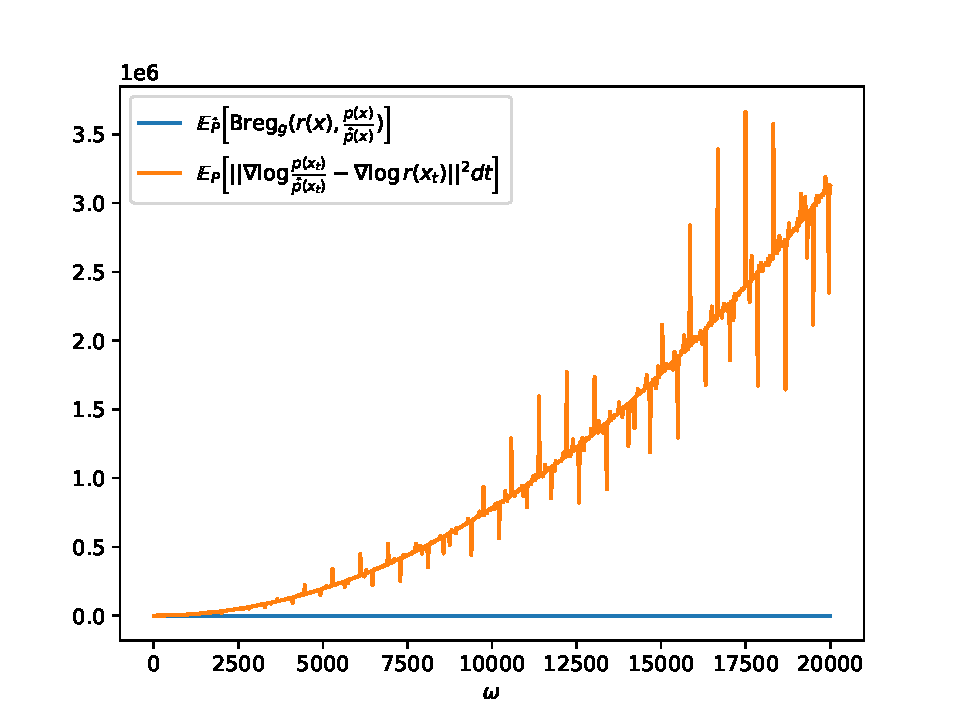
\includegraphics[width=0.8\linewidth]{gfx/1D_exple.pdf}
    \caption{1-dimensional example : Density ratio between two Gaussians, with a discriminator having an $\varepsilon$-optimal cross-entropy and a gain that goes to infinity}
    \label{fig:1Dexple}
\end{figure}







\subsection{Proof of Theorem~\ref{theorem:expectation_exploding}}\label{sec:app:proofoverfitting}


\begin{proof}
    Define the measures $\tilde{\mu}=\min\left(P,\hat{P}\right),\mu_{P}=\max\left(0,P-\hat{P}\right)$
    and $\mu_{\hat{P}}=\max\left(0,\hat{P}-P\right)$. Observe that $P=\tilde{\mu}+\mu_{P}$,
    $\hat{P}=\tilde{\mu}+\mu_{\hat{P}}$ and that $\tilde{\mu}\left(\mathbb{R}\right)=1-TV$
    where $TV$ is the total variation distance between $P$ and $\hat{P}$.
    Define the distribution $\mu=\frac{\tilde{\mu}}{\tilde{\mu}(\mathbb{R})}$
    and let $f_{\mu}$ and $f_{\tilde{\mu}}$ be the density of $\mu$
    and $\tilde{\mu}$ with respect to Lebesgue measure. Note that because
    $\tilde{\mu}$ is not normalized, $f_{\tilde{\mu}}$ does not integrate
    to one.
    
    Let us build two sets $S$ and $S'$ iteratively using the following
    rejection sampling procedure: First, start with $S=S'=\emptyset$.
    Then, for each $i$, add $x_{i}$ (respectively $x'_{i}$) to the
    set $S$ (respectively $S'$) with probability $\frac{f_{\tilde{\mu}}(x_{i})}{p(x_{i})}$
    (respectively $\frac{f_{\tilde{\mu}}(x'_{i})}{\hat{p}(x'_{i})}$).
    For now, denote $M_{1}=\left|S\right|$ and $M_{2}=\left|S'\right|$.
    It is easy to check using standard properties of rejection sampling
    that $\mathbb{E}\left[M_{1}\right]=\mathbb{E}\left[M_{2}\right]=N\times(1-TV)$.
    Finally, take the largest of both sets $S$ and $S'$ and remove its
    last added elements until both sets have same cardinality $M=\min\left(M_{1},M_{2}\right)$.
    Note that in all three sets $S$,$S'$ and $S\cup S'$, examples are
    distributed i.i.d. from $\mu$.
    
    Let us define the mean square error:
    
    \begin{align*}
    MSE & =\mathbb{E}_{x\sim P}\left[\left(\nabla_{x}d^{\star}(x)-\nabla_{x}d_{\phi}(x)\right)^{2}\right]\\
     & \ge\mathbb{E}\left[\left(\nabla_{x}d_{\phi}\right)^{2}\right]-2\mathbb{E}\left[\nabla_{x}d^{\star}.\nabla_{x}d_{\phi}\right]\\
     & \ge\mathbb{E}_{p}\left[\left(\nabla_{x}d_{\phi}\right)^{2}\right]-2\sqrt{\mathbb{E}_{p}\left[\left(\nabla_{x}d^{\star}\right)^{2}\right]}\sqrt{\mathbb{E}_{p}\left[\left(\nabla_{x}d_{\phi}\right)^{2}\right]}
    \end{align*}
    
    The last line follows from Cauchy-Schwartz inequality.
    
    We are interested into lower-bounding the \emph{expected} mean square
    error, noted $\mathbb{E}MSE$, where the expectation is over the training
    set $\left\{ x_{1},x_{1}'\ldots\right\} $ on which the discriminator
    $d_{\phi}$ is trained. So we would like to bound it.
    
    To derive this bound, we will first lower bound $\mathbb{E}_{p}\left[\left(\nabla_{x}d_{\phi}\right)^{2}\right]$.
    
    First, consider an arbitrary interval $B\subset\mathbb{R}$ of size
    $\beta$ containing at least one point $z\in S$ and one point $z'\in S'$
    such that $z<z'$.
    
    Then we can write
    
    \begin{align*}
    \int_{\mathbb{R}}\left(\nabla d_{\phi}\right)^{2}dP(x) & \ge\int_{B}\left(\nabla d_{\phi}\right)^{2}dP(x)\\
     & \ge\int_{B}\left(\nabla d_{\phi}\right)^{2}d\tilde{\mu}(x)=\int_{B}\left(\nabla d_{\phi}\right)^{2}f_{\tilde{\mu}}(x)dx\\
     & \ge\left(\inf_{x\in B}f_{\tilde{\mu}}(x)\right)\int_{B}\left(\nabla d_{\phi}\right)^{2}dx\\
     & \ge\left(\inf_{x\in B}f_{\tilde{\mu}}(x)\right)\int_{z}^{z'}\left(\nabla d_{\phi}\right)^{2}dx\\
     & =\left(\inf_{x\in B}f_{\tilde{\mu}}(x)\right)(z'-z)\int_{z}^{z'}\frac{\left(\nabla d_{\phi}\right)^{2}}{z'-z}dx\\
     & \ge\left(\inf_{x\in B}f_{\tilde{\mu}}(x)\right)(z'-z)\left(\int_{z}^{z'}\frac{\nabla d_{\phi}}{z'-z}dx\right)^{2}\text{ (by Jensen)}\\
     & =\frac{\inf_{x\in B}f_{\tilde{\mu}}(x)}{z'-z}\left(\int_{z}^{z'}\nabla d_{\phi}dx\right)^{2}\\
     & \ge\frac{\inf_{x\in B}f_{\tilde{\mu}}(x)}{\beta}\left(\int_{z}^{z'}\nabla d_{\phi}dx\right)^{2}
    \end{align*}
    
    Because both $p$ and $\hat{p}$ are L-Lipschitz, $f_{\tilde{\mu}}$
    has also this Lipschitz property. So for any $u\in B$ we have $f_{\tilde{\mu}}(u)-\inf_{x\in B}f_{\tilde{\mu}}(x)\le L\beta$,
    so $\inf_{x\in B}f_{\tilde{\mu}}(x)+L\beta\ge f_{\tilde{\mu}}(u)$,
    so $\inf_{x\in B}f_{\tilde{\mu}}(x)+L\beta\ge\frac{1}{\beta}\int_{B}f_{\tilde{\mu}}(x)dx=\frac{\tilde{\mu}\left(B\right)}{\beta}$.So
    we can write
    
    \[
    \int_{B}\nabla d_{\phi}^{2}dP(x)\ge\left(\frac{\tilde{\mu}\left(B\right)}{\beta^{2}}-L\right)\left(\int_{z}^{z'}\nabla d_{\phi}dx\right)^{2}
    \]
    
    Note that if $z>z'$ we would get by the same reasoning
    
    \[
    \int_{B}\nabla d_{\phi}^{2}dP(x)\ge\left(\frac{\tilde{\mu}\left(B\right)}{\beta^{2}}-L\right)\left(\int_{z'}^{z}\nabla d_{\phi}dx\right)^{2}
    \]
    
    To bound $\int_{z}^{z'}\nabla d_{\phi}dx$, recall that the cross-entropy
    for each $i$ is such that $\log\left(1+e^{-d_{\phi}(x_{i})}\right)\le\epsilon$
    and $\log\left(1+e^{d_{\phi}(x_{i}')}\right)\le\epsilon$. Thus,
    $1+e^{-d_{\phi}(x_{i})}\le e^{\epsilon}$ and $1+e^{d_{\phi}(x_{i}')}\le e^{\epsilon}$.
    So $d_{\phi}(x_{i})\ge\alpha$ and $d_{\phi}(x_{i}')\le-\alpha$
    where $\alpha=-\log\left(e^{\epsilon}-1\right)$. This also applies
    to $z$ and $z'$, so $\int_{\min(z,z')}^{\max(z,z')}\nabla d_{\phi}dx=\pm2\alpha$.
    Finally, we can summarize our findings by:
    
    \[
    \text{if both \ensuremath{S} and \ensuremath{S'} intersect with \ensuremath{B} then}\int_{B}\nabla d_{\phi}dP(x)\ge\left(\frac{\tilde{\mu}\left(B\right)}{\beta^{2}}-L\right)4\alpha^{2}
    \]
    
    Our goal now will be to show that there exists a small enough interval
    $B$ containing two points $z$ and $z'$ from $S$ and $S'$ with
    high probability.
    
    First, let us build an interval $A$ such that $\mu\left(A\right)\ge\frac{1}{2}$.
    By Chebyshev's inequality, we have that $\mu\left(\left\{ x:\left|x-\mathbb{E}_{\mu}x\right|\ge b\right\} \right)\le\frac{Var_{\mu}}{b^{2}}$
    for any $b$, so using the bound on the variance of lemma \ref{lem:variance_of_mu},
    we get that there exists a finite interval $A=\left[\mathbb{E}_{\mu}X-b,\mathbb{E}_{\mu}X+b\right]$
    where $b=\frac{\min\left(\sqrt{Var_{P}},\sqrt{Var_{\hat{P}}}\right)}{1-TV}$
    such that $\mu\left(A\right)\ge\frac{1}{2}$.
    
    Next, because $\mu(A)\ge\frac{1}{2}$, for any $0<\beta<2b$ there
    exists an interval $B\subset A$ of size $\beta$ such that $\mu\left(B\right)\ge\frac{\beta}{4b}$.
    Let us bound the probability that both $S$ and $S'$ intersect with
    $B$:
    
    \begin{align*}
    \mathbb{P}\left[B\cap S\neq\emptyset\wedge B\cap S'\neq\emptyset\right]= & 1-\mathbb{P}\left[B\cap S=\emptyset\vee B\cap S'=\emptyset\right]\\
    = & 1-\mathbb{P}\left[B\cap S=\emptyset\right]-\mathbb{P}\left[B\cap S'=\emptyset\right]+\mathbb{P}\left[B\cap S'=\emptyset\wedge B\cap S'=\emptyset\right]\\
    = & 1-\mu\left(\bar{B}\right)^{M}-\mu\left(\bar{B}\right)^{M}+\mu\left(\bar{B}\right)^{2M}\\
    \ge & 1-2\left(1-\mu\left(B\right)\right)^{M}\ge1-2\exp\left(-M\mu\left(B\right)\right)\\
    \ge & 1-2\exp\left(-\frac{M\beta}{4b}\right)
    \end{align*}
    
    For any non negative random variable $Z$, we know by the law of total
    expectation that $\mathbb{E}Z\ge\mathbb{E}\left[Z\mid condition\right]\mathbb{P}\left(condition\right)$,
    so in our case we have (here the expectation is over the dataset and
    the rejection sampling procedure):
    
    \begin{align*}
    \mathbb{E}\int_{B}\left(\nabla d_{\phi}\right)^{2}dP(x)\ge & \mathbb{E}\left[\int_{B}\left(\nabla d_{\phi}\right)^{2}dP(x)\mid B\cap S\neq\emptyset\wedge B\cap S'\neq\emptyset\right]\times\mathbb{P}\left[B\cap S\neq\emptyset\wedge B\cap S'\neq\emptyset\right]\\
    \ge & \left(\frac{\tilde{\mu}\left(B\right)}{\beta^{2}}-L\right)4\alpha^{2}\times\left(1-2\exp\left(-\frac{M\beta}{4b}\right)\right)\\
    \ge & \left(\frac{\mu\left(B\right)(1-TV)}{\beta^{2}}-L\right)4\alpha^{2}\times\left(1-2\exp\left(-\frac{M\beta}{4b}\right)\right)\\
    \ge & \left(\frac{1-TV}{4b\beta}-L\right)4\alpha^{2}\times\left(1-2\exp\left(-M\frac{\beta}{4b}\right)\right)
    \end{align*}
    
    Choosing $\beta=\frac{b}{M}4\log4$ we get a $\left(1-2\exp\left(-M\frac{\beta}{4b}\right)\right)=1/2$
    and 
    \begin{align*}
    \mathbb{E}\int_{B}\left(\nabla d_{\phi}\right)^{2}dP(x) & \ge\mathbb{E}\left(\frac{1-TV}{4b\beta}-L\right)2\alpha^{2}\\
     & =\left(\frac{(1-TV)\mathbb{E}\left[M\right]}{8b^{2}\log4}-2L\right)\left(\log\left(e^{\epsilon}-1\right)\right)^{2}
    \end{align*}
    
    It is known that $\mathbb{E}M=\mathbb{E}\min\left(M_{1},M_{2}\right)\ge\frac{1}{2}\mathbb{E}M_{1}=\frac{N\times(1-TV)}{2}$.
    So we finally get\\
    \begin{align*}
    \mathbb{E}\int_{\infty}\left(\nabla d_{\phi}\right)^{2}dP(x) & \ge\left(N\frac{(1-TV)^{2}}{16b^{2}\log4}-2L\right)\left(\log\left(e^{\epsilon}-1\right)\right)^{2}\\
     & =\left(N\frac{(1-TV)^{4}}{16\log4\min\left(Var_{P},Var_{\hat{P}}\right)}-2L\right)\left(\log\left(e^{\epsilon}-1\right)\right)^{2}
    \end{align*}
    
    Finally, we can bound the expected MSE:
    
    \begin{align*}
    \mathbb{E}MSE & \ge\mathbb{E}_{p}\left[\left(\nabla_{x}d_{\phi}\right)^{2}\right]-2\sqrt{\mathbb{E}_{p}\left[\left(\nabla_{x}d^{\star}\right)^{2}\right]}\sqrt{\mathbb{E}_{p}\left[\left(\nabla_{x}d_{\phi}\right)^{2}\right]}\\
     & \ge\mathbb{E}_{p}\left[\left(\nabla_{x}d_{\phi}\right)^{2}\right]-2\sqrt{\mathbb{E}_{p}\left[\left(\nabla_{x}d^{\star}\right)^{2}\right]}\sqrt{\mathbb{E}_{p}\left[\left(\nabla_{x}d_{\phi}\right)^{2}\right]}\\
    \end{align*}
    \end{proof}
    \begin{lemma}
    \label{lem:variance_of_mu}Let $P$ and $\hat{P}$ be two distributions
    over $\mathbb{R}$ and let $\tilde{\mu}=\min\left(P,\hat{P}\right)$.
    Then 
    \[
    Var_{\mu}\le\frac{1}{2(1-TV)^{2}}\min\left(Var_{P},Var_{\hat{P}}\right)
    \]
    \end{lemma}
    
    
    \begin{proof}
    Define $\mu=\frac{\tilde{\mu}}{\tilde{\mu}(\mathbb{R})}$. As before,
    $\mu=\frac{\tilde{\mu}}{1-TV}$, so we have
    
    \begin{align*}
    Var_{\mu} & =\mathbb{E}_{X\sim\mu}\left[(X-\mathbb{E}X)^{2}\right]=\frac{1}{2}\mathbb{E}_{X,X'\sim\mu}\left[(X-X')^{2}\right]\\
     & =\frac{1}{2}\int\int(x-x')^{2}d\mu(x)d\mu(x')\\
     & =\frac{1}{2(1-TV)^{2}}\int\int(x-x')^{2}d\tilde{\mu}(x)d\tilde{\mu}(x')\\
     & \le\frac{1}{2(1-TV)^{2}}\min\left(\int\int(x-x')^{2}dpdp,\int\int(x-x')^{2}d\hat{p}d\hat{p}\right)\\
     & =\frac{1}{2(1-TV)^{2}}\min\left(Var_{P},Var_{\hat{P}}\right)
    \end{align*}
    \end{proof}
    

    \subsection{Proof of Proposition~\ref{theorem:optimality_mse_sm}}\label{sec:app:proofmseloss}

\begin{proposition}
    Assume that $P$ and $\whP$ satisfy the assumptions detailed in Appendix~\ref{sec:appendix:assumptionssong}.
    Then, the following holds:
    \begin{equation}
        \argmin_\phi \calL_{\mathrm{SM}}^{d}(\phi) = \argmin_\phi \calL_{\mathrm{MSE}}^{d}(\phi).
    \end{equation} 
\end{proposition}
First, we can show that:
\begin{align}
    \calL_{\mathrm{MSE}}^{d}(\phi) =& \int_0^T\lambda(t)   \E_{P_0, P_{t\vert\vx_0}}\left[\Vert \nabla_{\vx_t} \log p_t(\vx_t\vert\vx_0) - \nabla_{\vx_t} \log \whp_t(\vx_t) - \nabla_{\vx_t} \vd_\phi(\vx_t, t)\Vert_2^2 \right]\dt \\
    =& \begin{aligned}[t]
        \int_0^T&\lambda(t) \E_{P_t}\left[\frac{1}{2}\left\Vert\nabla_{\vx_t} \vd_\phi(\vx_t, t)\right\Vert_2^2\right] \dt \\
        &+ \int_0^T\lambda(t) \E_{P_0, P_{t\vert\vx_0}}\left[\left\langle \nabla_{\vx_t}d(\vx_t, t), \nabla_{\vx_t} \log \frac{p_t(\vx_t\vert\vx_0)}{\whp_t(\vx_t)}\right\rangle\right] \dt \\
        &+ \int_0^T\lambda(t) \E_{P_0, P_{t\vert\vx_0}}\left[\frac{1}{2}\left\Vert\nabla_{\vx_t} \log \frac{p_t(\vx_t\vert\vx_0)}{\whp_t(\vx)}\right\Vert_2^2\right] \dt 
    \end{aligned}\\
    =& \int_0^T\lambda(t) \E_{P_t}\left[\frac{1}{2}\left\Vert\nabla_{\vx_t} \vd_\phi(\vx_t, t)\right\Vert_2^2\right] \dt + J(\phi) + C_1,
\end{align}
where $C_1$ is a constant independent of $\phi$. And we can write $J$ as:
\begin{align}
    J(\phi) =& \int_0^T\lambda(t) \E_{P_0, P_{t\vert\vx_0}}\left[\left\langle \nabla_{\vx_t}d(\vx_t, t), \nabla_{\vx_t} \log \frac{p_t(\vx_t\vert\vx_0)}{\whp_t(\vx_t)}\right\rangle\right] \dt \\
    =& \begin{aligned}[t]
       \int_0^T&\lambda(t) E_{P_0, P_{t\vert\vx_0}}\left[\left\langle \nabla_{\vx_t}d(\vx_t, t), \nabla_{\vx_t} \log p_t(\vx_t\vert\vx_0)\right\rangle\right] \dt \\
        &- \int_0^T\lambda(t) E_{P_0, P_{t\vert\vx_0}}\left[\left\langle \nabla_{\vx_t}d(\vx_t, t), \nabla_{\vx_t} \log \whp_t(\vx_t)\right\rangle\right] \dt. 
    \end{aligned} 
\end{align}
Using the result of \citep{vincent_connection_2011}, we can show the term in the first integral can be rewritten as:
\begin{align}
    E_{P_0, P_{t\vert\vx_0}}\left[\left\langle \nabla_{\vx_t}d(\vx_t, t), \nabla_{\vx_t} \log p_t(\vx_t\vert\vx_0)\right\rangle\right] =  E_{P_t}\left[\left\langle \nabla_{\vx_t}d_\phi(\vx_t, t), \nabla_{\vx_t} \log p_t(\vx_t)\right\rangle\right].
\end{align}
Thus, we can rewrite $J$ as:
\begin{align}
    J(\phi) =& \begin{aligned}[t]
        \int_0^T&\lambda(t) E_{P_t}\left[\left\langle \nabla_{\vx_t}d_\phi(\vx_t, t), \nabla_{\vx_t} \log p_t(\vx_t)\right\rangle\right] \dt \\
        &- \int_0^T\lambda(t) E_{P_0, P_{t\vert\vx_0}}\left[\left\langle \nabla_{\vx_t}d(\vx_t, t), \nabla_{\vx_t} \log \whp_t(\vx_t)\right\rangle\right] \dt
    \end{aligned} \\
    = & \int_0^T\lambda(t) E_{P_t}\left[\left\langle \nabla_{\vx_t}d_\phi(\vx_t, t),\nabla_{\vx_t} \log \frac{p_t(\vx_t)}{\whp(\vx_t)}\right\rangle\right] \dt.\label{eq:J}
\end{align}
And on the other side, we have:
\begin{align}
    \calL_{SM}^d(\phi) =& \int_0^T\lambda(t) \E_{P_t}\left[\Vert \nabla_{\vx_t} \vd_\phi(\vx_t, t)\Vert_2^2\right] \dt \\
    =& \begin{aligned}[t]
        \int_0^T&\lambda(t) \E_{P_t}\left[\frac{1}{2}\left\Vert\nabla_{\vx_t} \vd_\phi(\vx_t, t)\right\Vert_2^2\right] \dt \\
        &+ \int_0^T\lambda(t) \E_{P_t}\left[\left\langle \nabla_{\vx_t}d(\vx_t, t), \nabla_{\vx_t} \log \frac{p_t(\vx_t)}{\whp_t(\vx_t)}\right\rangle\right] \dt \\
        &+ \int_0^T\lambda(t) \E_{P_t}\left[\frac{1}{2}\left\Vert\nabla_{\vx_t} \log \frac{p_t(\vx_t)}{\whp_t(\vx_t)}\right\Vert_2^2\right] \dt
    \end{aligned} \\
    =& \int_0^T\lambda(t) \E_{P_t}\left[\frac{1}{2}\left\Vert\nabla_{\vx_t} \vd_\phi(\vx_t, t)\right\Vert_2^2\right] \dt + J(\phi) + C_2 
\end{align}
using Equation~\eqref{eq:J} and $C_2$ is a constant independent of $\phi$. Thus, we have $\calL_{\mathrm{MSE}}^{d}(\phi) = \calL_{\mathrm{SM}}^{d}(\phi) + C_3$, where $C_3$ is a constant independent of $\phi$. Thus, the minimizer of $\calL_{\mathrm{MSE}}^{d}(\phi)$ is the same as the minimizer of $\calL_{\mathrm{SM}}^{d}(\phi)$.